

%To run this example, follow the link
View demo code of this section: \demonotebook{05}{5.4_DC_QAOA}

\subsubsection{Background}
In the field of quantum computing, researchers are continuously seeking efficient and robust methods to tackle complex problems. Adiabatic Quantum Computation (AQC) is one such approach, where a quantum system evolves gradually from an initial Hamiltonian to a final Hamiltonian that encodes the desired solution. According to the adiabatic theorem, if this evolution is slow enough, the system will remain in the ground state of the Hamiltonian throughout the process:
\begin{equation}
    H(t) = (1-\lambda(t))H_{\text{initial}} + \lambda(t)H_{\text{final}},
\end{equation}
where \(\lambda(t) \in [0, 1]\). However, conducting AQC in practical scenarios faces challenges arising from external noise, imperfections, and the need for long evolution times. To overcome these limitations and enhance the efficiency of adiabatic evolution, one promising approach is the Quantum Approximate Optimization Algorithm (QAOA).

QAOA employs a parameterized quantum circuit to prepare a trial state that approximates solutions for optimization problems. By optimizing the ansatz parameters, QAOA seeks to find the optimal values that minimize the objective function, which encodes the problem's energy landscape. This method allows for shorter evolution times and can be more resilient to noise and imperfections, making it a viable alternative to AQC for practical quantum computing applications.

However, hardware implementations of QAOA face challenges due to noise, decoherence, and the complexity of parameter optimization. To enhance its performance and robustness, the Digitized Counterdiabatic Quantum Approximate Optimization Algorithm (DC-QAOA) introduces the counterdiabatic (CD) term:

\begin{equation}
    H_{\text{DC-QAOA}} = H_{\text{initial}}(\gamma) + H_{\text{final}}(\beta) + H_{\text{CD}}(\alpha),
\end{equation}

This approach combines ideas from both Adiabatic Quantum Computation (AQC) and QAOA by introducing an additional parameter per layer compared to QAOA, resulting in shallower quantum circuits without compromising accuracy:
\begin{equation}
    \label{eq:evo operator}
    U(\gamma, \beta) \to U(\gamma, \beta, \alpha), \quad F(\gamma, \beta) \to F(\gamma, \beta, \alpha),
\end{equation}
where \(\alpha\), \(\beta\), and \(\gamma\) represent the digitized parameters, \(F\) is the cost function, and \(U\) is the evolution operator.

The CD term acts as an additional component in the Hamiltonian, designed based on the instantaneous eigenstates and eigenenergies of the evolving Hamiltonian. It effectively suppresses errors and reduces the required evolution time, leading to enhanced efficiency and reliability in quantum computations.

To derive the precise form of the counterdiabatic term, various techniques, such as Lewis-Riesenfeld invariants and transitionless quantum driving~\cite{PhysRevA.83.062116}, have been applied. The implementation of the CD term is tailored to the specific problem and dynamics of the quantum system, utilizing available control techniques. When obtaining exact CD terms is challenging, an approximate CD driving approach is proposed, utilizing the nested commutator method  with the adiabatic gauge potential~\cite{PhysRevResearch.4.013141}:

\begin{equation}
    A_{\lambda}^{(l)} = i \sum_{k=1}^{l} \alpha_{k}(t) [H_{a}, [H_{a}, \ldots, [H_{a}, \partial_{\lambda} H_{a}]]].
\end{equation}

DC-QAOA holds promise for solving a wide range of optimization problems, from combinatorial optimization to protein folding~\cite{PhysRevApplied.20.014024} and financial portfolio optimization~\cite{PhysRevResearch.4.043204}. As quantum computing technology continues to advance, DC-QAOA represents an exciting avenue for leveraging the counterdiabatic term and parameter space digitization to unlock new frontiers in quantum optimization.

\textbf{Target problem}
\begin{itemize}
    \item[1.] Learn how to find the ground state of problem Hamiltonian
    \item[2.] Utilize quantum circuits to find optimized parameters
\end{itemize}
\textbf{Required Mindquantum functionalities}
\begin{itemize}
    \item[1.] gradient-based optimizer
    \item[2.] Batch quantum circuit simulator

\end{itemize}

\subsubsection{Implement}
As a mature variant of variational algorithm, this method requires two steps, which is building the ansatz circuit and optimization. Now let's look at how to implement DC-QAOA into the Ising model~\cite{PhysRevResearch.4.013141}. The general form of the Hamiltonian is given by the following equation:

\begin{equation}
    H_{final} = H_{prob} = -J_{ij}\sum_{i=1}^{n-1}\sigma^z_i\sigma^z_{i+1}-h_{i}\sum_{i=1}^{n}{\sigma_i^z} + k_{i}\sum_{i=1}^{n}\sigma_{i}^{x}.
\end{equation}

The initial state is chosen as $H_{initial} = \sum_{i}\sigma_{i}^{x}$, which should drives transitions between different states, facilitating the exploration of the solution space. To be specific, we choose longitudinal field Ising model (LFIM) Hamiltonian, in which $J_{ij}=1,~h_{i}=1,~k_{i}=0$.
\begin{lstlisting}
# Generate H_{initial} as H_{mixer}.
# n_qubits is the number of qubits
def generate_h_mixer(n_qubits:int):
    h_mixer = QubitOperator()
    for i in range(n_qubits):
        h_mixer += QubitOperator(f'X{i}')
    return h_mixer

# Generate H_{final} as H_{prob}.
def generate_h_prob(n_qubits:int, J:float, h:float):
    h_prob = QubitOperator()
    for i in range(n_qubits-1):
        h_prob += QubitOperator(f'Z{i} Z{i+1}', -J)
    for i in range(n_qubits):
        h_prob += QubitOperator(f'Z{i}', -h)
    return h_prob
\end{lstlisting}

In our case,  a pool of CD operators is defined using the nested commutator approach of the adiabatic gauge potential~\cite{PhysRevResearch.6.013147}
$$A = \{\sigma^{y},\sigma^{z}\sigma^{y}, \sigma^{y}\sigma^{z}, \sigma^{x}\sigma^{y}, \sigma^{y}\sigma^{x} \}.$$
Here we present a 12 qubits system and we consider CD term to be  $A^{*} = \sum_{i=1}^{n}\sigma_{i}^{y}$. Following we build an ansatz layer for DC-QAOA.
\begin{lstlisting}
def generate_h_cd(n_qubits:int):
    h_cd = QubitOperator()
    for i in range(n_qubits):
        h_cd += QubitOperator(f'Y{i}')
    return h_cd
\end{lstlisting}

\begin{lstlisting}
n_qubits = 12
J, h = 1, 1

h_prob = generate_h_prob(n_qubits, J, h)
h_mixer = generate_h_mixer(n_qubits)
h_cd = generate_h_cd(n_qubits)
\end{lstlisting}

In order to prepare the eigenstates for $H_{initial}$, we first put ${\rm prep\_circ}$, and then apply the evolution operator on it.
\begin{lstlisting}
# Prepare the eigenstates for $H_{mixer}$.
prep_circ = UN(H, n_qubits)
# Choose the number of layers p.
p = 1

ansatz_template =   u_p + u_m  + u_cd

ansatz = Circuit() + prep_circ

for i in range(p):
    ansatz += add_suffix(ansatz_template, str(i)) + BarrierGate()
\end{lstlisting}

As long as we have set up the ansatz circuit, we can change the number of layers or type of classical optimizer in order to find the optimal parameter set. We define the cost function using
\begin{equation}
    F(\alpha,~\beta,~\gamma) = \left<\psi_0\right|U^{\dagger}\ H_{prob} U\left|\psi_0\right>,
\end{equation}
where $U = \Pi_{i=0}^p U_{cd}(\alpha_i)U_m(\beta_i)U_p(\gamma_i)$ and this is just the evolution operator in Eq.~\ref{eq:evo operator}.
\begin{lstlisting}
def train(ham, ansatze, iteration):

    # bulid the quantum circuit

    circ = ansatze
    sim = Simulator('mqvector', ansatze.n_qubits)

    grad_ops = sim.get_expectation_with_grad(ham, circ)
    net = MQAnsatzOnlyLayer(grad_ops)
    opti = nn.Adagrad(net.trainable_params(), learning_rate=0.05)
    train_net = nn.TrainOneStepCell(net, opti)

    result = []
    for i in range(iteration):
        train_net()
        result.append(np.array(train_net()[0]))
    pr = dict(zip(ansatze.params_name, net.weight.asnumpy()))

    return result
\end{lstlisting}

In this tutorial, we will optimize the gradient using Adam optimizer~\cite{PhysRevResearch.6.013147}, which will have good enough results. If you plot the figure of mean energy, you will have Fig.~\ref{fig:dc}. Here, the dashed green line is the exact eigenvalue of $H_{prob}$, the solid blue line is the mean value of one-layer-DC-QAOA during the optimizing process, and the solid orange line is QAOA with one layer. We can notice that DC-QAOA has converged to the exact value in 20 steps while QAOA is trapped in the local minimal. Comparing these two algorithms from the ability to estimate the ground state, DC-QAOA has an advantage over QAOA.
\begin{figure}
    \centering
    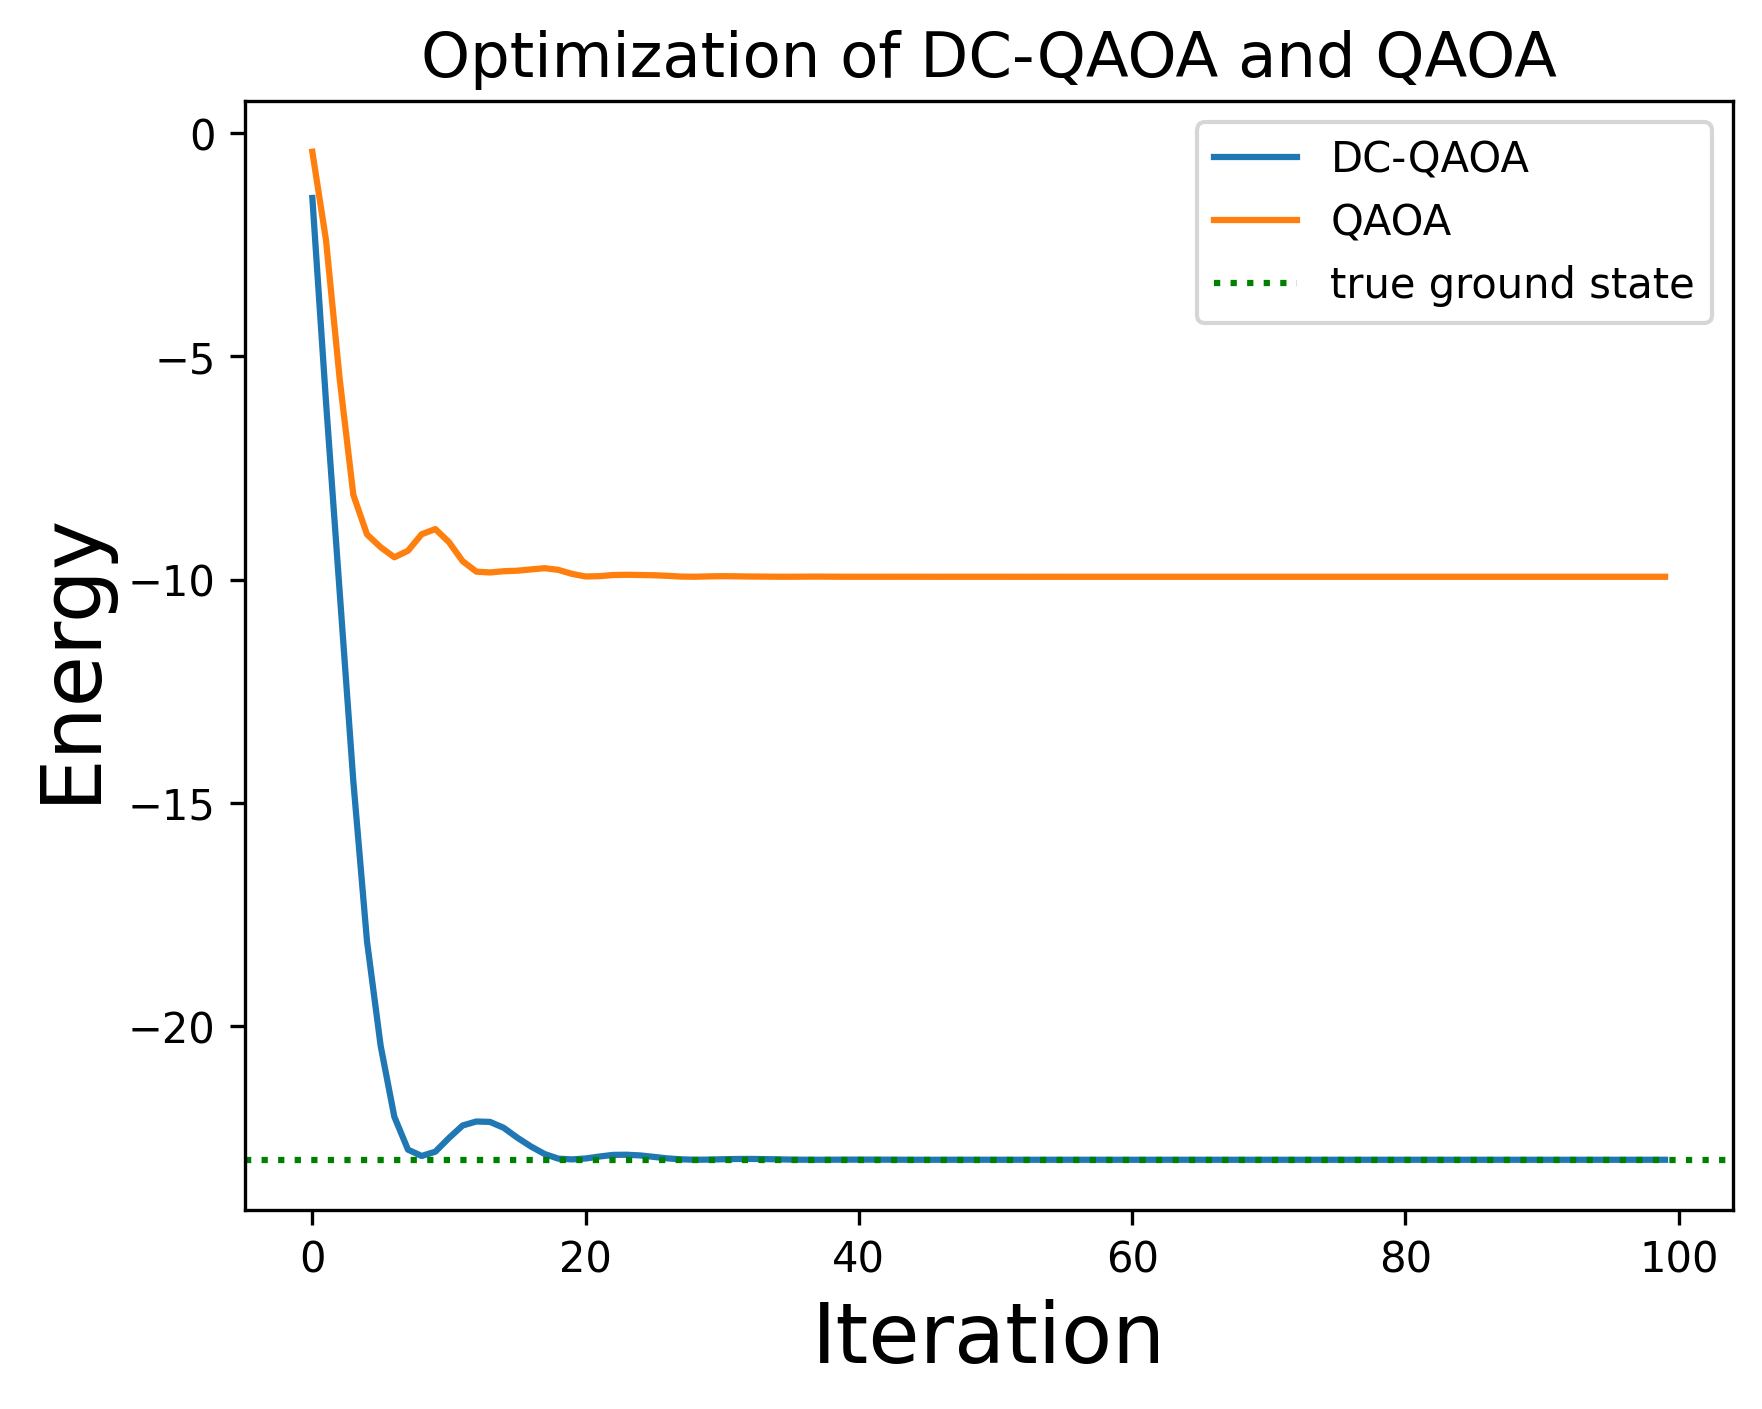
\includegraphics[width = 1 \linewidth]{5.4.1_figure/DC-QAOA.png}
    \caption{Energy as the function of iterations.}
    \label{fig:dc}
\end{figure}